\documentclass[12pt]{letter}
\usepackage{geometry}
  \geometry{
  a4paper,
  total={210mm,297mm},
  left=0mm,
  right=0mm,
  bottom=0mm,
  top=10mm
}
\usepackage{tikz}
\usepackage{fdsymbol} %var suits
\usepackage{wasysym} %smiley

\newcommand{\diamonds}{\color{red}$\vardiamondsuit$\color{black}} 
\newcommand{\hearts}{\color{red}$\varheartsuit$\color{black}} 
\newcommand{\clubs}{$\clubsuit$} 
\newcommand{\spades}{$\spadesuit$}
\newcommand{\card}[9]
{
  \parbox[c][29mm]{20mm}{\scalebox{3}{\centering #1}}
  \parbox[c][29mm]{20mm}{\scalebox{3}{\centering #2}}
  \parbox[c][29mm]{20mm}{\scalebox{3}{\centering #3}}

  \parbox[c][29mm]{10mm}{\scalebox{3}{\centering #4}}
  \parbox[c][29mm]{25mm}{\scalebox{3}{\centering #5}}
  \parbox[c][29mm]{20mm}{\scalebox{3}{\centering #6}}

  \parbox[c][29mm]{10mm}{\scalebox{3}{\centering #7}} 
  \parbox[c][29mm]{10mm}{\scalebox{3}{\centering #8}} 
  \parbox[c][29mm]{20mm}{\scalebox{3}{\centering #9}}
}


\begin{document}

\begin{minipage}[t]{69mm}
  \centering
  \begin{tikzpicture}
    [
      very thick,
      rounded corners=20pt,
      card/.style=
      {
        align=center,
        text width=64mm,
        inner sep=0pt,
        minimum height=89mm,
        minimum width=64mm,
        text centered,
        fill=white,
        text=black,
        draw,
      },
      txt/.style=
      {
        align=center,
        text width=64mm,
        inner sep=0pt,
        minimum height=10mm,
        minimum width=64mm,
        text centered,
        text=black,
        font=\small\sffamily\bfseries
      }
    ],
    \node[card](TheCard)
    {
      \card{~ \large \diamonds}
            {~ }
            {~ }
            {~ }
            {~ \huge \diamonds}
            {~ }
            {~ }
            {~ }
            {~ \large \diamonds}
    };
    \node[txt, below of=TheCard, node distance=89mm](TheTitle)
    {
      %title here
    };
  \end{tikzpicture}
\end{minipage}
\begin{minipage}[t]{69mm}
  \centering
  \begin{tikzpicture}
    [
      very thick,
      rounded corners=20pt,
      card/.style=
      {
        align=center,
        text width=64mm,
        inner sep=0pt,
        minimum height=89mm,
        minimum width=64mm,
        text centered,
        fill=white,
        text=black,
        draw,
      },
      txt/.style=
      {
        align=center,
        text width=64mm,
        inner sep=0pt,
        minimum height=10mm,
        minimum width=64mm,
        text centered,
        text=black,
        font=\small\sffamily\bfseries
      }
    ],
    \node[card](TheCard)
    {
      \card{~ \large \diamonds}
            {~ }
            {~ }
            {~ }
            {~ \huge \diamonds}
            {~ }
            {~ }
            {~ }
            {~ \large \diamonds}
    };
    \node[txt, below of=TheCard, node distance=89mm](TheTitle)
    {
      %title here
    };
  \end{tikzpicture}
\end{minipage}
\begin{minipage}[t]{69mm}
  \centering
  \begin{tikzpicture}
    [
      very thick,
      rounded corners=20pt,
      card/.style=
      {
        align=center,
        text width=64mm,
        inner sep=0pt,
        minimum height=89mm,
        minimum width=64mm,
        text centered,
        fill=white,
        text=black,
        draw,
      },
      txt/.style=
      {
        align=center,
        text width=64mm,
        inner sep=0pt,
        minimum height=10mm,
        minimum width=64mm,
        text centered,
        text=black,
        font=\small\sffamily\bfseries
      }
    ],
    \node[card](TheCard)
    {
      \card{~ \large \hearts}
            {~ }
            {~ }
            {~ }
            {~ \huge \hearts}
            {~ }
            {~ }
            {~ }
            {~ \large \hearts}
    };
    \node[txt, below of=TheCard, node distance=89mm](TheTitle)
    {
      %title here
    };
  \end{tikzpicture}
\end{minipage}


\vspace*{-140pt}\begin{minipage}[t]{69mm}
  \centering
  \begin{tikzpicture}
    [
      very thick,
      rounded corners=20pt,
      card/.style=
      {
        align=center,
        text width=64mm,
        inner sep=0pt,
        minimum height=89mm,
        minimum width=64mm,
        text centered,
        fill=white,
        text=black,
        draw,
      },
      txt/.style=
      {
        align=center,
        text width=64mm,
        inner sep=0pt,
        minimum height=10mm,
        minimum width=64mm,
        text centered,
        text=black,
        font=\small\sffamily\bfseries
      }
    ],
    \node[card](TheCard)
    {
      \card{~ \large \hearts}
            {~ }
            {~ }
            {~ }
            {~ \huge \hearts}
            {~ }
            {~ }
            {~ }
            {~ \large \hearts}
    };
    \node[txt, below of=TheCard, node distance=89mm](TheTitle)
    {
      %title here
    };
  \end{tikzpicture}
\end{minipage}
\begin{minipage}[t]{69mm}
  \centering
  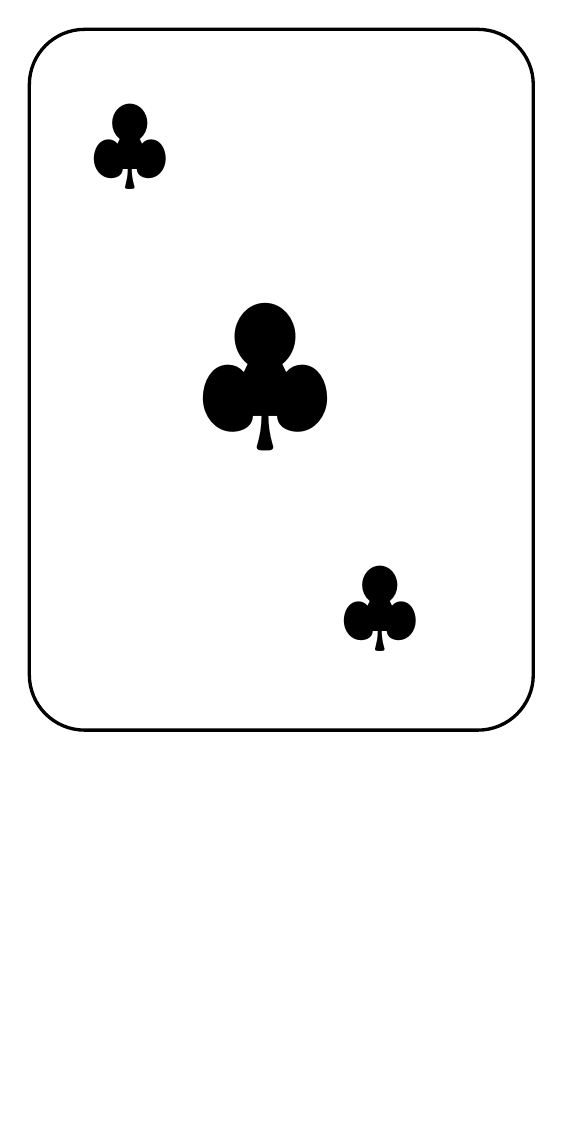
\begin{tikzpicture}
    [
      very thick,
      rounded corners=20pt,
      card/.style=
      {
        align=center,
        text width=64mm,
        inner sep=0pt,
        minimum height=89mm,
        minimum width=64mm,
        text centered,
        fill=white,
        text=black,
        draw,
      },
      txt/.style=
      {
        align=center,
        text width=64mm,
        inner sep=0pt,
        minimum height=10mm,
        minimum width=64mm,
        text centered,
        text=black,
        font=\small\sffamily\bfseries
      }
    ],
    \node[card](TheCard)
    {
      \card{~ \large \clubs}
            {~ }
            {~ }
            {~ }
            {~ \huge \clubs}
            {~ }
            {~ }
            {~ }
            {~ \large \clubs}
    };
    \node[txt, below of=TheCard, node distance=89mm](TheTitle)
    {
      %title here
    };
  \end{tikzpicture}
\end{minipage}
\begin{minipage}[t]{69mm}
  \centering
  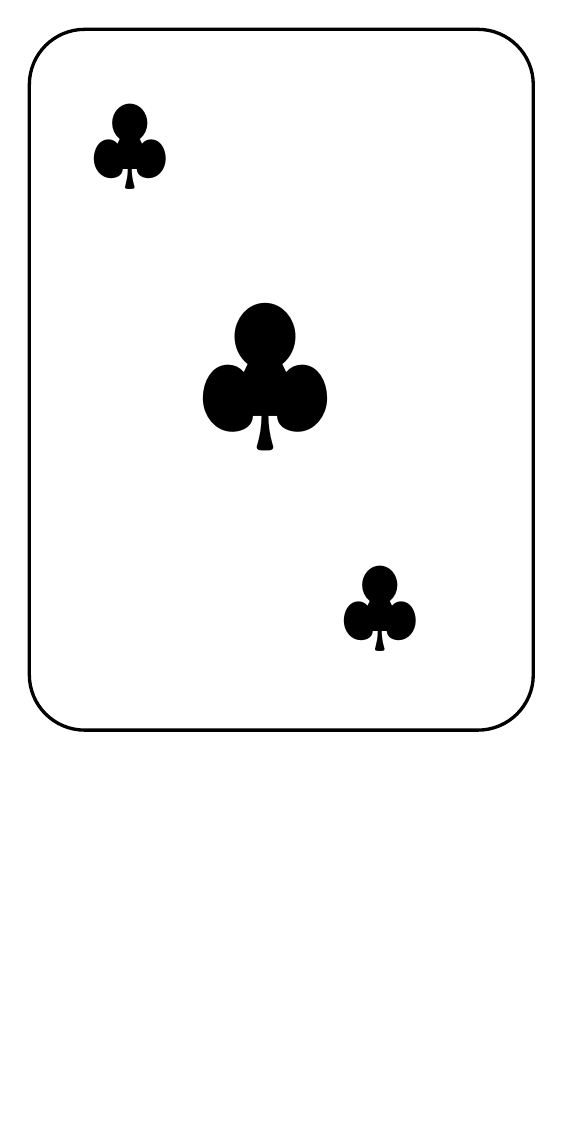
\begin{tikzpicture}
    [
      very thick,
      rounded corners=20pt,
      card/.style=
      {
        align=center,
        text width=64mm,
        inner sep=0pt,
        minimum height=89mm,
        minimum width=64mm,
        text centered,
        fill=white,
        text=black,
        draw,
      },
      txt/.style=
      {
        align=center,
        text width=64mm,
        inner sep=0pt,
        minimum height=10mm,
        minimum width=64mm,
        text centered,
        text=black,
        font=\small\sffamily\bfseries
      }
    ],
    \node[card](TheCard)
    {
      \card{~ \large \clubs}
            {~ }
            {~ }
            {~ }
            {~ \huge \clubs}
            {~ }
            {~ }
            {~ }
            {~ \large \clubs}
    };
    \node[txt, below of=TheCard, node distance=89mm](TheTitle)
    {
      %title here
    };
  \end{tikzpicture}
\end{minipage}


\vspace*{-140pt}\begin{minipage}[t]{69mm}
  \centering
  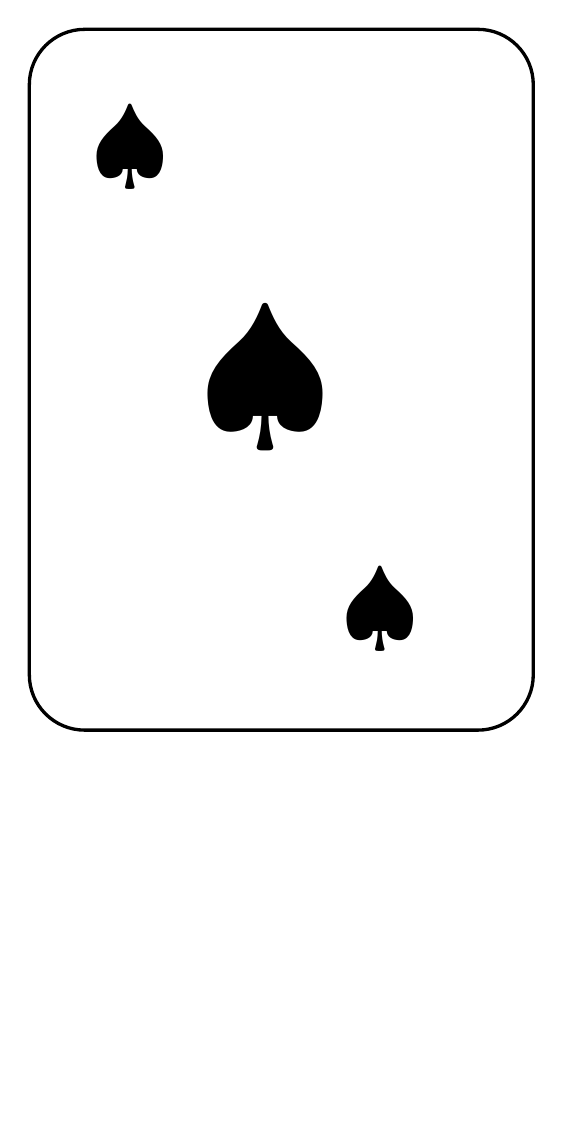
\begin{tikzpicture}
    [
      very thick,
      rounded corners=20pt,
      card/.style=
      {
        align=center,
        text width=64mm,
        inner sep=0pt,
        minimum height=89mm,
        minimum width=64mm,
        text centered,
        fill=white,
        text=black,
        draw,
      },
      txt/.style=
      {
        align=center,
        text width=64mm,
        inner sep=0pt,
        minimum height=10mm,
        minimum width=64mm,
        text centered,
        text=black,
        font=\small\sffamily\bfseries
      }
    ],
    \node[card](TheCard)
    {
      \card{~ \large \spades}
            {~ }
            {~ }
            {~ }
            {~ \huge \spades}
            {~ }
            {~ }
            {~ }
            {~ \large \spades}
    };
    \node[txt, below of=TheCard, node distance=89mm](TheTitle)
    {
      %title here
    };
  \end{tikzpicture}
\end{minipage}
\begin{minipage}[t]{69mm}
  \centering
  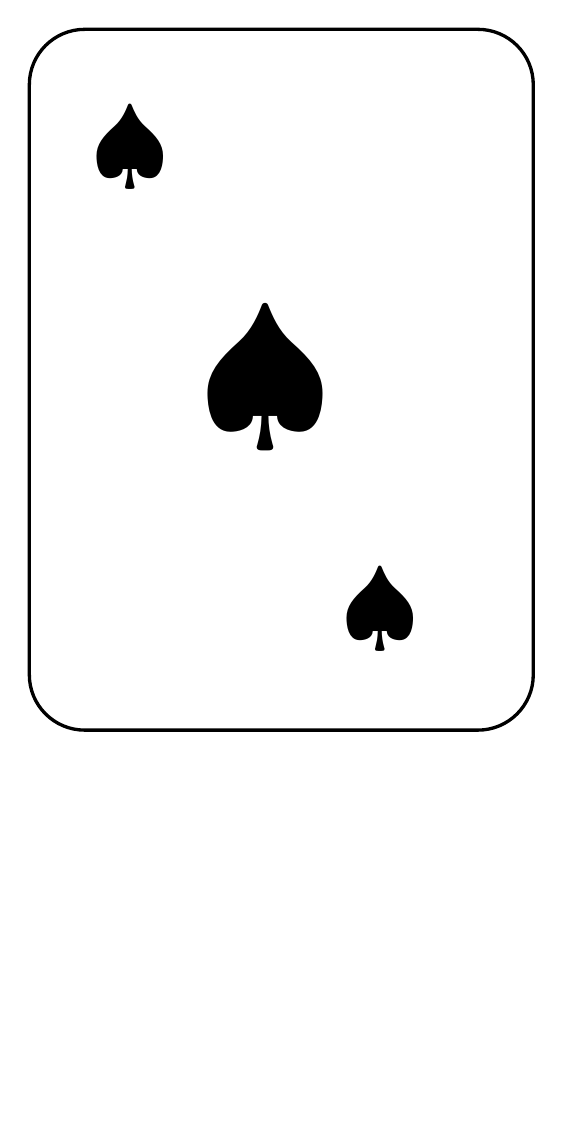
\begin{tikzpicture}
    [
      very thick,
      rounded corners=20pt,
      card/.style=
      {
        align=center,
        text width=64mm,
        inner sep=0pt,
        minimum height=89mm,
        minimum width=64mm,
        text centered,
        fill=white,
        text=black,
        draw,
      },
      txt/.style=
      {
        align=center,
        text width=64mm,
        inner sep=0pt,
        minimum height=10mm,
        minimum width=64mm,
        text centered,
        text=black,
        font=\small\sffamily\bfseries
      }
    ],
    \node[card](TheCard)
    {
      \card{~ \large \spades}
            {~ }
            {~ }
            {~ }
            {~ \huge \spades}
            {~ }
            {~ }
            {~ }
            {~ \large \spades}
    };
    \node[txt, below of=TheCard, node distance=89mm](TheTitle)
    {
      %title here
    };
  \end{tikzpicture}
\end{minipage}
\begin{minipage}[t]{69mm}
  \centering
  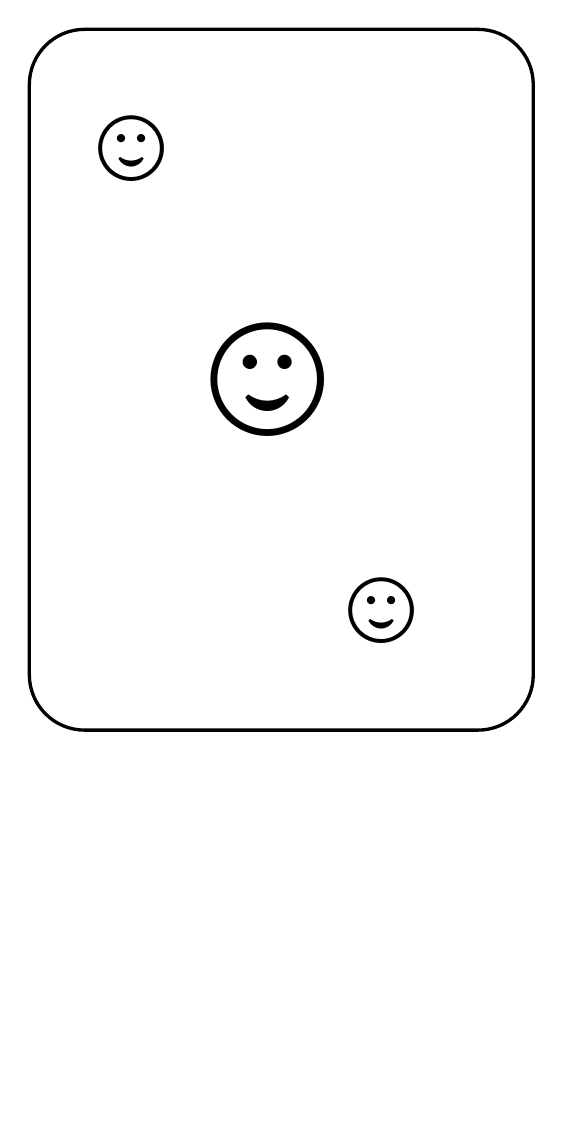
\begin{tikzpicture}
    [
      very thick,
      rounded corners=20pt,
      card/.style=
      {
        align=center,
        text width=64mm,
        inner sep=0pt,
        minimum height=89mm,
        minimum width=64mm,
        text centered,
        fill=white,
        text=black,
        draw,
      },
      txt/.style=
      {
        align=center,
        text width=64mm,
        inner sep=0pt,
        minimum height=10mm,
        minimum width=64mm,
        text centered,
        text=black,
        font=\small\sffamily\bfseries
      }
    ],
    \node[card](TheCard)
    {
      \card{~ \large \smiley}
            {~ }
            {~ }
            {~ }
            {~ \huge \smiley}
            {~ }
            {~ }
            {~ }
            {~ \large \smiley}
    };
    \node[txt, below of=TheCard, node distance=89mm](TheTitle)
    {
      %title here
    };
  \end{tikzpicture}
\end{minipage}


\vspace*{-140pt}\clearpage\end{document}